\documentclass[11pt]{article}
\usepackage[margin=1in]{geometry}
\usepackage{amsmath,amssymb}
\usepackage{booktabs}
\usepackage{siunitx}
\usepackage{hyperref}
\usepackage{graphicx}
\usepackage{epstopdf}
\usepackage{caption}
\usepackage{xcolor}
\usepackage{array}

\sisetup{
  separate-uncertainty = true,
  per-mode = symbol,
}

\title{R2: Cross-Code Validation of the UH MkV FEL\\
  Beamline Optimisation}
\author{Eremey Valetov}
\date{4 March 2026}

\graphicspath{{../../../../backend/test/}}

\begin{document}
\maketitle

\section{Introduction}

The UH MkV FEL transport line (118~elements, 23~quadrupoles) was
optimised independently using three simulation codes with distinct
physics models: FELsim (linear transfer matrices), COSY~INFINITY
(differential algebra maps with fringe fields), and RF-Track (full
particle tracking).  Achieving agreement required identifying and
correcting implementation errors in each code's adapter layer.  This
report documents the corrections applied, presents the cross-code
comparison at $\varepsilon_n = 8\;\pi\cdot\text{mm}\cdot\text{mrad}$,
and benchmarks the optimisation algorithms.

The undulator Twiss targets follow Weinberg, Fisher \&
Li~\cite{weinberg2025}: $\beta_x = \SI{1.400}{m}$,
$\alpha_x = 0.470$, $\beta_y = \SI{0.242}{m}$, $\alpha_y = 0$.  The
11-stage sequential optimisation decomposes the 23-quadrupole problem
into physically motivated sections (doublets, triplets, chromaticity
quads).


\section{Simulation Codes}

\paragraph{FELsim} uses $4\times4$ linear transfer matrices with
analytical dipole models: sector-bend bodies with a triangle-rule
fringe correction for vertical edge kicks.  The optimiser is
Nelder-Mead (NM) with multi-start for Stage~11.
$E = \SI{40}{MeV}$, 500~particles, seed = 42.

\paragraph{COSY INFINITY} uses differential algebra (DA) to compute
transfer maps to arbitrary order.  The optimiser is the built-in
gradient-based FIT (algorithm~1), which exploits DA derivatives.
Two fringe field settings were tested: FR\,0 (hard-edge, no fringe)
and FR\,1 (first-order Enge-model fringe, warm-started from FR\,0).
Computation order~3, 3~DA dimensions (6D phase space).

\paragraph{RF-Track} (v2.5.5, CERN) performs element-by-element
particle tracking through the beamline.  Twiss parameters are computed
from tracked particle distributions.  The optimiser is NM with prefix
caching: elements~0--87 are tracked once, and only the Stage~11 suffix
(elements~87--118) is re-tracked per NM evaluation.


\section{Model Corrections and Bug Fixes}

Achieving cross-code agreement required identifying and correcting
errors in each code's interface.  Table~\ref{tab:fixes} summarises the
corrections.

\begin{table}[ht]
\centering
\caption{Bug fixes and model corrections enabling cross-code agreement.}
\label{tab:fixes}
\small
\begin{tabular}{@{} l l l @{}}
\toprule
Code & Issue & Fix \\
\midrule
FELsim     & DPW edge-kick sign inversion        & $R = L/|\theta|$ (unsigned) \\
RF-Track   & \texttt{SBend} P/$\delta$ confusion  & Analytical sector-bend correction \\
RF-Track   & DPW modelled as \texttt{Drift(L)}    & Thin-lens quad for edge kicks \\
RF-Track   & Edge-kick sign (signed $K_0$)        & $K_0 = |\theta|/L$ \\
RF-Track   & $R_{12}$ unit conversion error        & R-matrix invariant under scaling \\
RF-Track   & Coord5 ct$\to$l conversion (C7)      & Corrected sign and scaling \\
COSY       & Initial $\beta_0 = 1$~m default      & $\beta_0 = \sigma^2/\varepsilon \approx \SI{6.34}{m}$ \\
COSY       & Individual FIT objectives reset       & Combined MSE objective \\
COSY       & FR\,1 cold-start failure              & Warm-start from FR\,0 solution \\
\bottomrule
\end{tabular}
\end{table}


\subsection{FELsim: DPW Edge-Kick Sign}

FELsim's \texttt{dipole\_wedge} class computed the bending radius as
$R = L/\theta$, using the signed bending angle.  For negative-angle
chicane dipoles ($\theta < 0$), this inverted $R$, flipping the sign
of the vertical edge kicks.  The fix replaces $R = L/\theta$ with
$R = L/|\theta|$.  All prior optimisation results involving chicane
dipoles were invalidated by this bug.


\subsection{RF-Track Adapter Corrections}

Five issues were identified and resolved in the RF-Track adapter.

\paragraph{SBend P/$\delta$ confusion.}
RF-Track's \texttt{SBend(L, angle, P\_Q)} constructor interprets the
bunch's absolute momentum $P$ (MeV/$c$, 6th column of \texttt{Bunch6d})
as the momentum deviation $\delta = \Delta P/P_0$, producing
$\sim$\SI{910}{mm} displacement.  The setter-only \texttt{set\_K0} has
no effect.  We implemented an analytical workaround: dipole bodies are
tracked as \texttt{Drift(L)}, and the correction matrix
$M_\text{sector} \times M_\text{drift}^{-1}$ is applied to $(x, x')$,
with dispersion ($R_{16}$, $R_{26}$) and path-length ($R_{56}$) terms
added.  The correction is exact for the sector-bend transfer matrix
(verified to 6~decimal places).

\paragraph{DPW modelling.}
The adapter converted dipole wedges to \texttt{Drift(L)} with the
physical wedge length ($\approx$\SI{10}{mm}), adding spurious position
propagation.  Replaced with thin-lens \texttt{Quadrupole(L=1e-10,
K1L=$-|K_0|\tan\eta$)} for edge kicks.

\paragraph{Edge-kick sign.}
The \texttt{\_annotate\_dipole\_edges()} method used signed
$K_0 = \theta/L$, inverting edge kicks for negative-angle chicane
dipoles.  Fixed to $K_0 = |\theta|/L$.

\paragraph{R-matrix units.}
Erroneous $\times 1000$ scaling of $R_{12}$ and $\div 1000$ scaling of
$R_{21}$ when converting between (m,\,rad) and (mm,\,mrad) coordinates.
The R-matrix is invariant under this coordinate scaling because both
position and angle scale by the same factor.

\paragraph{Coordinate conversion (C7).}
The FELsim$\leftrightarrow$RF-Track coordinate conversion for the 5th
phase-space coordinate (ct vs $l$) had incorrect sign and scaling,
inflating the initial $\sigma(\text{ct})$ by $9.5\times$.  This
invalidated all longitudinal RF-Track results prior to the C7 fix.


\subsection{COSY INFINITY Adapter Corrections}

\paragraph{Initial Twiss.}
The initial beta function must be computed from the beam distribution:
$\beta_0 = \sigma_x^2/\varepsilon \approx \SI{6.34}{m}$ (where
$\sigma_x = \SI{0.8}{mm}$, $\varepsilon = \SI{0.101}{\pi.mm.mrad}$).
Using the common default $\beta_0 = \SI{1}{m}$ produces completely
incorrect transport ($\alpha_x = -2.8$ instead of $\approx 0$ after
Stage~1).

\paragraph{Combined MSE objective.}
COSY's FIT with individual objectives (\texttt{ENDFIT} with multiple
\texttt{OBJ}) resets all variables when \emph{any} single objective
fails to converge.  A combined MSE objective preserves DA derivatives
for gradient-based optimisation and converges monotonically.

\paragraph{Warm-starting for fringe fields.}
Running FR\,1 from default initial guesses fails
(MSE~$\approx 0.2$) because the changed dipole edge kicks push the
sequential FIT stages into incompatible local minima.  Using the
converged FR\,0 currents as initial values for FR\,1 resolves this:
MSE~$= 7.9 \times 10^{-8}$ with $\Delta I_\text{max} = \SI{0.76}{A}$.


\section{Cross-Code Baseline Results}

Table~\ref{tab:baseline} compares the optimised Twiss parameters at
the undulator entrance for $\varepsilon_n = 8\;\pi\cdot\text{mm}\cdot\text{mrad}$.
All codes match the targets in the $x$-plane.  The $\beta_y$ residual
in RF-Track ($0.055$ vs target $0.242$~m) arises from the missing
triangle-rule fringe correction $\phi$ in the thin-lens edge-kick model.

\begin{table}[ht]
\centering
\caption{Cross-code comparison at $\varepsilon_n = 8\;\pi\cdot\text{mm}\cdot\text{mrad}$,
  $\sigma_E = 0.5\%$.  Targets: $\beta_x = \SI{1.400}{m}$,
  $\alpha_x = 0.470$, $\beta_y = \SI{0.242}{m}$, $\alpha_y = 0$.}
\label{tab:baseline}
\begin{tabular}{@{} l l S[scientific-notation=true]
  S[round-precision=4] S[round-precision=4]
  S[round-precision=4] S[round-precision=4] @{}}
\toprule
Code & Model & {MSE} & {$\beta_x$ (m)} & {$\alpha_x$}
  & {$\beta_y$ (m)} & {$\alpha_y$} \\
\midrule
FELsim NM    & Transfer matrix     & 1.20e-06 & 1.4000 & 0.4700 & 0.2418 & -0.0000 \\
COSY FR\,0   & DA map (no fringe)  & 2.27e-07 & 1.3996 & 0.4700 & 0.2412 & -0.0006 \\
COSY FR\,1   & DA map (1st fringe) & 3.65e-09 & 1.4000 & 0.4700 & 0.2418 &  0.0001 \\
RF-Track opt & Particle tracking   & 7.02e-03 & 1.4010 & 0.4628 & 0.0548 & -0.0028 \\
\bottomrule
\end{tabular}
\end{table}

FELsim NM and COSY (FR\,0, FR\,1) achieve MSEs of $10^{-6}$--$10^{-9}$,
matching all four Twiss targets to within $10^{-3}$.  COSY's
gradient-based DA optimiser converges $\sim 10^3\times$ more precisely
than NM\@.  RF-Track's higher MSE ($7.0 \times 10^{-3}$) reflects the
systematic $\beta_y$ deficit from the thin-lens edge-kick model, not
optimizer limitations.

Figure~\ref{fig:twiss} shows the Twiss comparison graphically.


\section{Quadrupole Current Comparison}

Table~\ref{tab:currents} compares the optimised quadrupole currents
across all four runs.  Stages~1--2 and 6--9 show excellent agreement
($\Delta < \SI{0.1}{A}$).  The principal discrepancy is Stage~5
(double triplet): COSY finds a negative-polarity local minimum
($I_{35}, I_{37} < 0$), inaccessible to FELsim's bounded NM
($I \in [0, 10]$~A).  Stage~11 currents differ across all codes
because the models produce different edge kicks in the final triplet
section.

\begin{table}[ht]
\centering
\caption{Optimised quadrupole currents: FELsim NM, COSY FR\,0,
  COSY FR\,1 (warm-started), and RF-Track opt (Stage~11 only).}
\label{tab:currents}
\small
\sisetup{table-format=+1.3}
\begin{tabular}{@{} c l c SSSS c @{}}
\toprule
{Elem} & {Label} & {F/D} & {FELsim (A)} & {COSY FR\,0 (A)} & {COSY FR\,1 (A)} & {RFT-opt (A)} & {Stage} \\
\midrule
1   & LQ1   & F &  0.822 &  0.839 &  0.842 & {---} & 1 \\
3   & LQ2   & D &  1.043 &  1.052 &  1.057 & {---} & 1 \\
10  & DPHQ  & F &  3.883 &  3.957 &  3.979 & {---} & 2 \\
16  & F1QA  & D &  2.240 &  1.993 &  1.994 & {---} & 3 \\
18  & F1QB  & F &  4.953 &  4.859 &  4.955 & {---} & 3 \\
20  & F1QC  & D &  3.426 &  3.499 &  3.599 & {---} & 3 \\
27  & DPHQ  & F &  4.666 &  4.685 &  4.711 & {---} & 4 \\
33  & F2QA  & D &  2.694 &  0.357 &  0.518 & {---} & 5 \\
35  & F2QB  & F &  2.652 & -1.975 & -1.849 & {---} & 5 \\
37  & F2QC  & D &  0.277 & -1.995 & -1.985 & {---} & 5 \\
50  & DPHQ  & F &  4.674 &  4.685 &  4.696 & {---} & 6 \\
56  & F3QA  & D &  3.122 &  3.168 &  3.218 & {---} & 7 \\
58  & F3QB  & F &  3.313 &  3.321 &  3.361 & {---} & 7 \\
61  & F3QC  & F &  5.178 &  5.166 &  5.252 & {---} & 8 \\
63  & F3QD  & D &  4.043 &  4.011 &  4.080 & {---} & 8 \\
70  & DPHQ  & F &  4.682 &  4.662 &  4.811 & {---} & 9 \\
76  & F4QA  & D &  3.934 &  3.869 &  3.953 & {---} & 10 \\
78  & F4QB  & F &  4.079 &  4.452 &  4.506 & {---} & 10 \\
80  & F4QC  & D &  0.014 &  0.608 &  0.592 & {---} & 10 \\
87  & DPHQ  & F &  1.362 &  1.259 &  1.610 &  2.045 & 11 \\
93  & UBQ1  & D &  0.945 &  2.348 &  2.473 &  1.405 & 11 \\
95  & UBQ2  & F &  2.885 &  3.802 &  3.602 &  0.722 & 11 \\
97  & UBQ3  & D &  2.192 &  4.747 &  3.995 &  0.111 & 11 \\
\bottomrule
\end{tabular}
\end{table}

Despite the different Stage~11 currents, all codes match the undulator
Twiss targets.  The different optimal currents reflect genuine model
differences --- each code finds the best solution within its own physics.
Direct current injection between codes (using one code's optimised
currents in another) produces poor results (RFT-val MSE~$= 2.0$ at
$\varepsilon_n = 8$) because the accumulated edge-kick differences
shift the beamline state at the undulator entrance.


\section{Single-Dipole Transfer Matrix Comparison}

Table~\ref{tab:sandwich} compares the vertical edge kick $M_{43}$
for individual DPW-DPH-DPW dipole sandwiches.  The discrepancy
grows with bending angle: 3.9\% at $1.5^\circ$, 8.9\% at $4^\circ$,
and 10\% at $11.25^\circ$ (FR\,0 vs FELsim).  The \texttt{FC} Enge
coefficients for the FC1/FC2 chicane produce 76\% weaker $y$-kicks,
indicating that realistic fringe fields partially cancel the geometric
edge focusing.

\begin{table}[ht]
\centering
\caption{Vertical edge kick $M_{43}$ (rad/m) and Y-plane stability
  for representative dipole triplets.}
\label{tab:sandwich}
\small
\begin{tabular}{@{} l c SSSS @{}}
\toprule
{Dipole} & {$\theta$ ($^\circ$)} & {FELsim} & {COSY FR\,0} & {COSY FR\,3} & {COSY FR\,3+FC} \\
\midrule
\multicolumn{6}{@{}l}{\emph{$M_{43}$ (vertical kick, rad/m)}} \\
Transport  & 1.5   & -7.42e-3 & -7.71e-3 & -6.78e-3 & {---} \\
Chicane    & 4.0   & -1.11e-1 & -1.21e-1 & -8.93e-2 & {---} \\
FC1        & 11.25 & -9.50e-1 & -1.04e+0 & -7.79e-1 & -2.27e-1 \\
\midrule
\multicolumn{6}{@{}l}{\emph{$|\mathrm{Tr}(M_y)/2|$ (stability, $<1$ required)}} \\
Transport  & 1.5   & 0.9997 & 0.9997 & 0.9997 & {---} \\
Chicane    & 4.0   & 0.9977 & 0.9975 & 0.9982 & {---} \\
FC1        & 11.25 & 0.9823 & 0.9805 & 0.9855 & 0.9957 \\
\bottomrule
\end{tabular}
\end{table}


\section{Parameter Sensitivity}

Table~\ref{tab:sensitivity} summarises the S4 parameter scans
(energy spread, chirp, emittance) using the MSE quality thresholds:
Excellent ($< 10^{-3}$), Acceptable ($< 0.01$), Marginal ($< 0.1$),
Failed ($\geq 0.1$).  The optimisation is robust across typical
operating ranges.  The only failure occurs at extreme emittance values
($\varepsilon_n \leq 2$ or $\varepsilon_n = 5$, where NM is trapped
in a local minimum).

\begin{table}[ht]
\centering
\caption{Quality distribution across S4 parameter scans (FELsim NM).}
\label{tab:sensitivity}
\begin{tabular}{@{} l c c cccc SS @{}}
\toprule
Scan & Range & $N$ & Exc. & Acc. & Mar. & Fail
  & {Best MSE} & {Worst MSE} \\
\midrule
$\sigma_E$ (\%)         & 0.1--5 & 15 & 14 & 1 & 0 & 0 & 8.52e-07 & 1.08e-03 \\
$h$ (s$^{-1}$)          & 0--4e10 & 12 & 12 & 0 & 0 & 0 & 1.32e-06 & 2.28e-04 \\
$\varepsilon_n$ (mm mrad) & 1--20 & 10 & 6 & 3 & 0 & 1 & 1.20e-06 & 2.39e+01 \\
\bottomrule
\end{tabular}
\end{table}

Figure~\ref{fig:mse_param} shows the MSE vs parameter for all three
scans.


\section{Optimiser Comparison}

Two evolutionary optimiser configurations (glyfada) were benchmarked
against NM for Stage~11 at three emittance points.  Table~\ref{tab:opt}
compares the MSE values.  COSY FIT results are included as a reference
for the best achievable MSE at each emittance.

\subsection{W6: Glyfada ULS (Uniform Random)}

The initial benchmark (W6) used glyfada's default ULS algorithm with
uniform random initialisation over the full parameter space
($[0, 15] \times [0, 10]^3$), 30$\times$20 = 600~evaluations.
NM outperforms by 3--6 orders of magnitude at all emittance points.
At $\varepsilon_n = 5$, all 600 evaluations return the penalty value
(unstable optics).

\subsection{W7: Glyfada CMA-ES (Warm-Started)}

A re-benchmark (W7) used CMA-ES with warm-starting from the NM
solution, informed bounds ($\pm$\SI{3}{A} around NM), feasibility-rules
constraint handling, and $5\times$ more evaluations (600 total).
Despite these improvements, CMA-ES still fails catastrophically:
MSE~$= 7.7 \times 10^5$ at $\varepsilon_n = 5$ and MSE~$= 17.8$ at
$\varepsilon_n = 8$.

\begin{table}[ht]
\centering
\caption{Stage~11 optimiser comparison across emittance points.
  COSY FIT uses gradient-based DA optimisation; FELsim NM uses
  Nelder-Mead with 5~restarts; Glyfada ULS and CMA-ES use
  evolutionary search.}
\label{tab:opt}
\begin{tabular}{@{} c S[scientific-notation=true] S[scientific-notation=true]
  S[scientific-notation=true] S[scientific-notation=true] @{}}
\toprule
{$\varepsilon_n$} & {COSY FIT} & {FELsim NM} & {Glyfada ULS} & {Glyfada CMA-ES} \\
\midrule
5  & 1.40e-02 & 4.02e-01 & 1.00e+06 & 7.73e+05 \\
8  & 2.27e-07 & 1.20e-06 & 2.96e+00 & 1.78e+01 \\
14 & 1.44e-08 & 1.09e-03 & 3.11e-01 & 2.56e+00 \\
\bottomrule
\end{tabular}
\end{table}

The FELsim MSE landscape has an extremely narrow feasibility basin:
large regions of the 4D parameter space produce divergent optics.
Evolutionary search cannot navigate this landscape efficiently, even
with warm-starting and tight bounds.  The gradient-based COSY FIT
(exploiting DA derivatives) is the most effective optimiser, followed
by NM with multi-start.

Figure~\ref{fig:opt_mse} shows the MSE comparison graphically.


\section{Summary}

\begin{enumerate}
  \item \textbf{Three-code agreement achieved.}  FELsim, COSY~INFINITY,
    and RF-Track independently match the undulator Twiss targets at
    $\varepsilon_n = 8$, with MSEs ranging from $3.7 \times 10^{-9}$
    (COSY FR\,1) to $7.0 \times 10^{-3}$ (RF-Track).
    Table~\ref{tab:baseline} and Fig.~\ref{fig:twiss}.

  \item \textbf{Nine bugs fixed across three codes} (Table~\ref{tab:fixes}).
    The most critical were the FELsim DPW edge-kick sign, the RF-Track
    SBend P/$\delta$ confusion, and the COSY initial Twiss computation.
    All prior chicane-related optimisation results were invalidated.

  \item \textbf{Different quad currents, same Twiss.}  Each code
    converges to a different set of Stage~11 currents because the
    physics models produce different dipole edge kicks
    (Table~\ref{tab:currents}).  Direct current injection between codes
    fails; each code must optimise within its own model.

  \item \textbf{Dipole model is the dominant source of discrepancy.}
    Single-dipole comparisons show 4--20\% differences in the vertical
    edge kick depending on bending angle and fringe field model
    (Table~\ref{tab:sandwich}).

  \item \textbf{Optimisation is robust} across energy spread (0.1--5\%)
    and chirp (0--$4\times10^{10}$\,s$^{-1}$), with MSE~$< 10^{-3}$
    everywhere except extreme emittance values
    (Table~\ref{tab:sensitivity}).

  \item \textbf{Gradient-based optimisation (COSY FIT) outperforms
    all others.}  Evolutionary search (glyfada) fails at every emittance
    point by 3--6 orders of magnitude vs NM, even with CMA-ES,
    warm-starting, and tight bounds (Table~\ref{tab:opt}).  The narrow
    feasibility basin of the FELsim MSE landscape makes evolutionary
    approaches ineffective for this problem.
\end{enumerate}


\section*{Figures}

\begin{figure}[p]
  \centering
  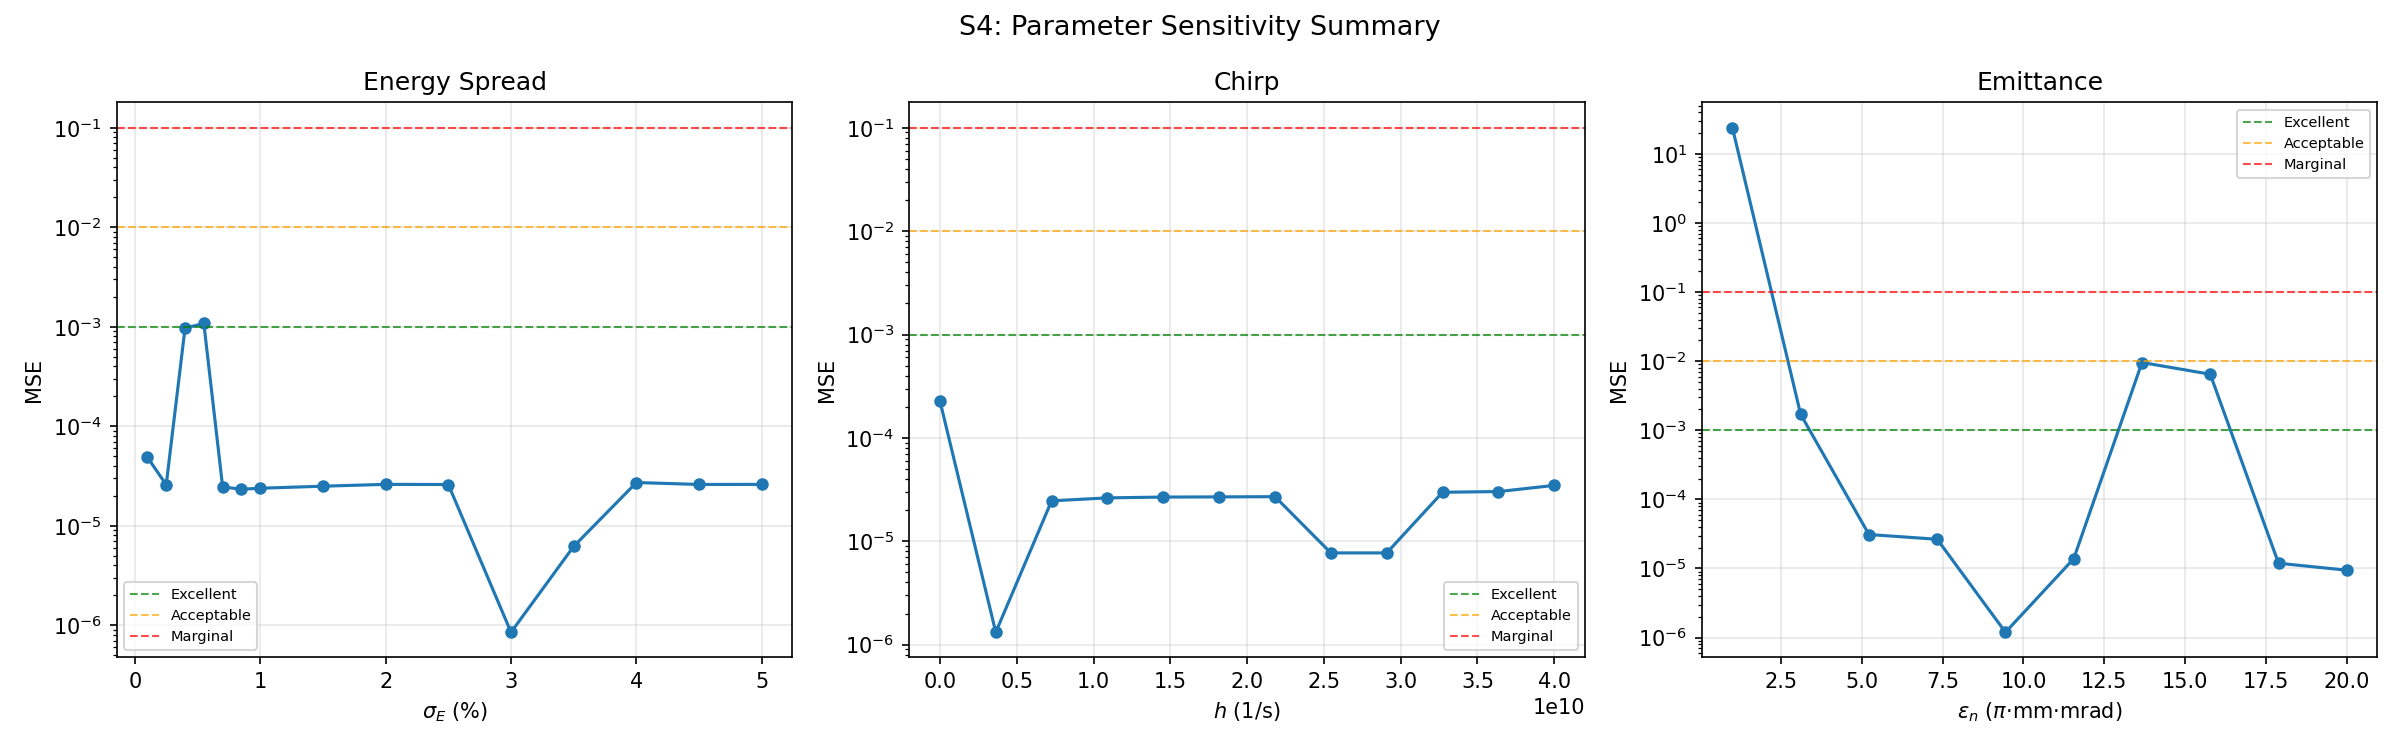
\includegraphics[width=\textwidth]{results/R2/R2_mse_vs_parameter}
  \caption{MSE vs parameter for the S4 sensitivity scans: energy spread
    (left), chirp (centre), emittance (right).  The dashed lines
    indicate quality thresholds.}
  \label{fig:mse_param}
\end{figure}

\begin{figure}[p]
  \centering
  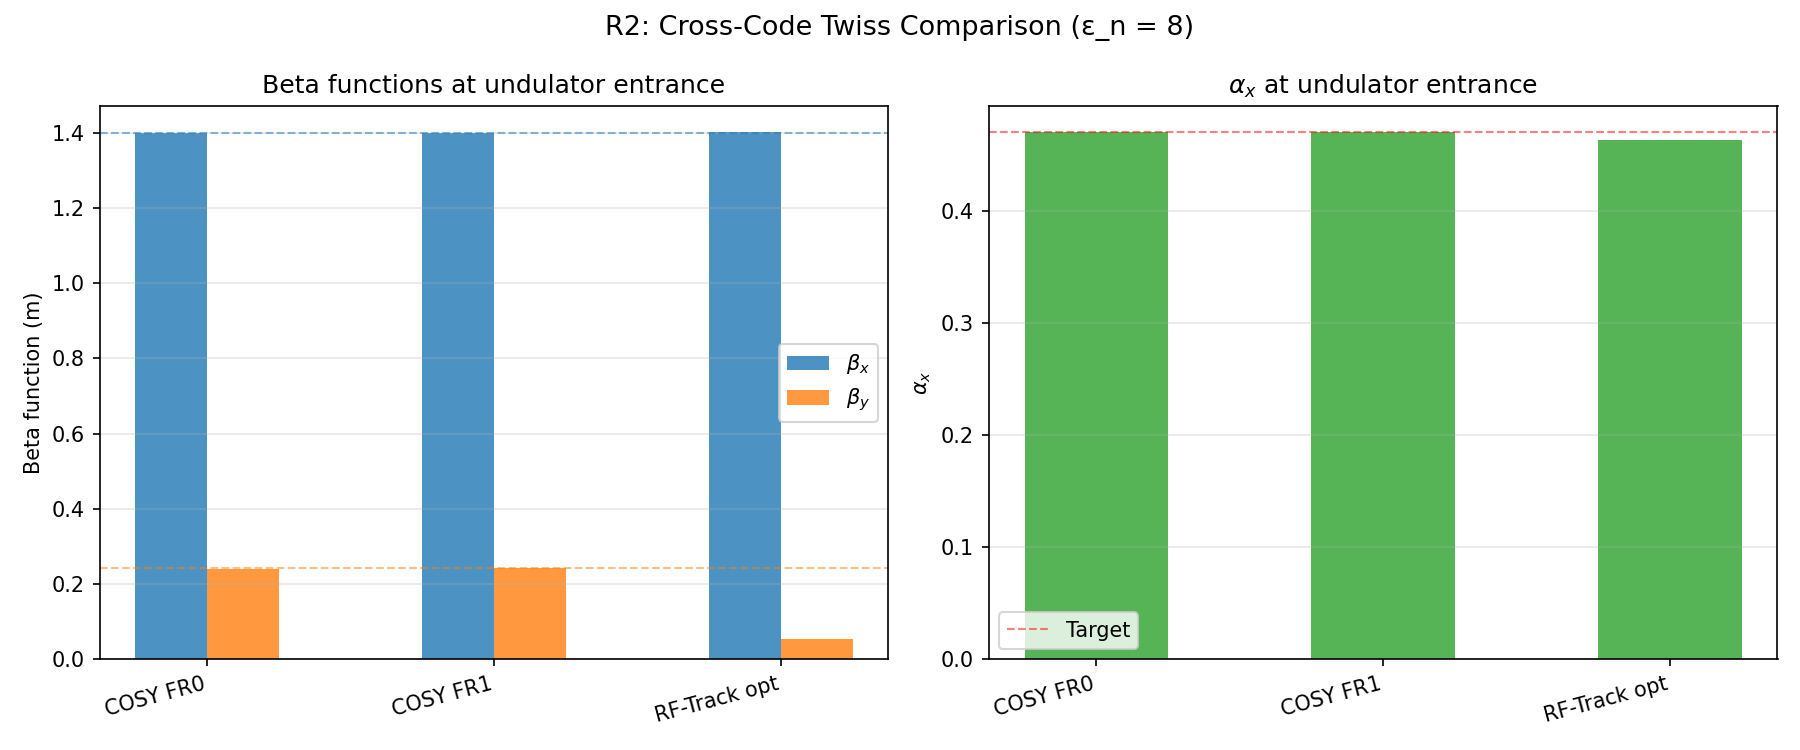
\includegraphics[width=0.85\textwidth]{results/R2/R2_cross_code_twiss}
  \caption{Cross-code Twiss comparison at $\varepsilon_n = 8$.  All
    codes match $\beta_x$ and $\alpha_x$ closely.  RF-Track's $\beta_y$
    deficit (0.055 vs 0.242~m) is due to the missing triangle-rule
    fringe correction in the thin-lens edge-kick model.}
  \label{fig:twiss}
\end{figure}

\begin{figure}[p]
  \centering
  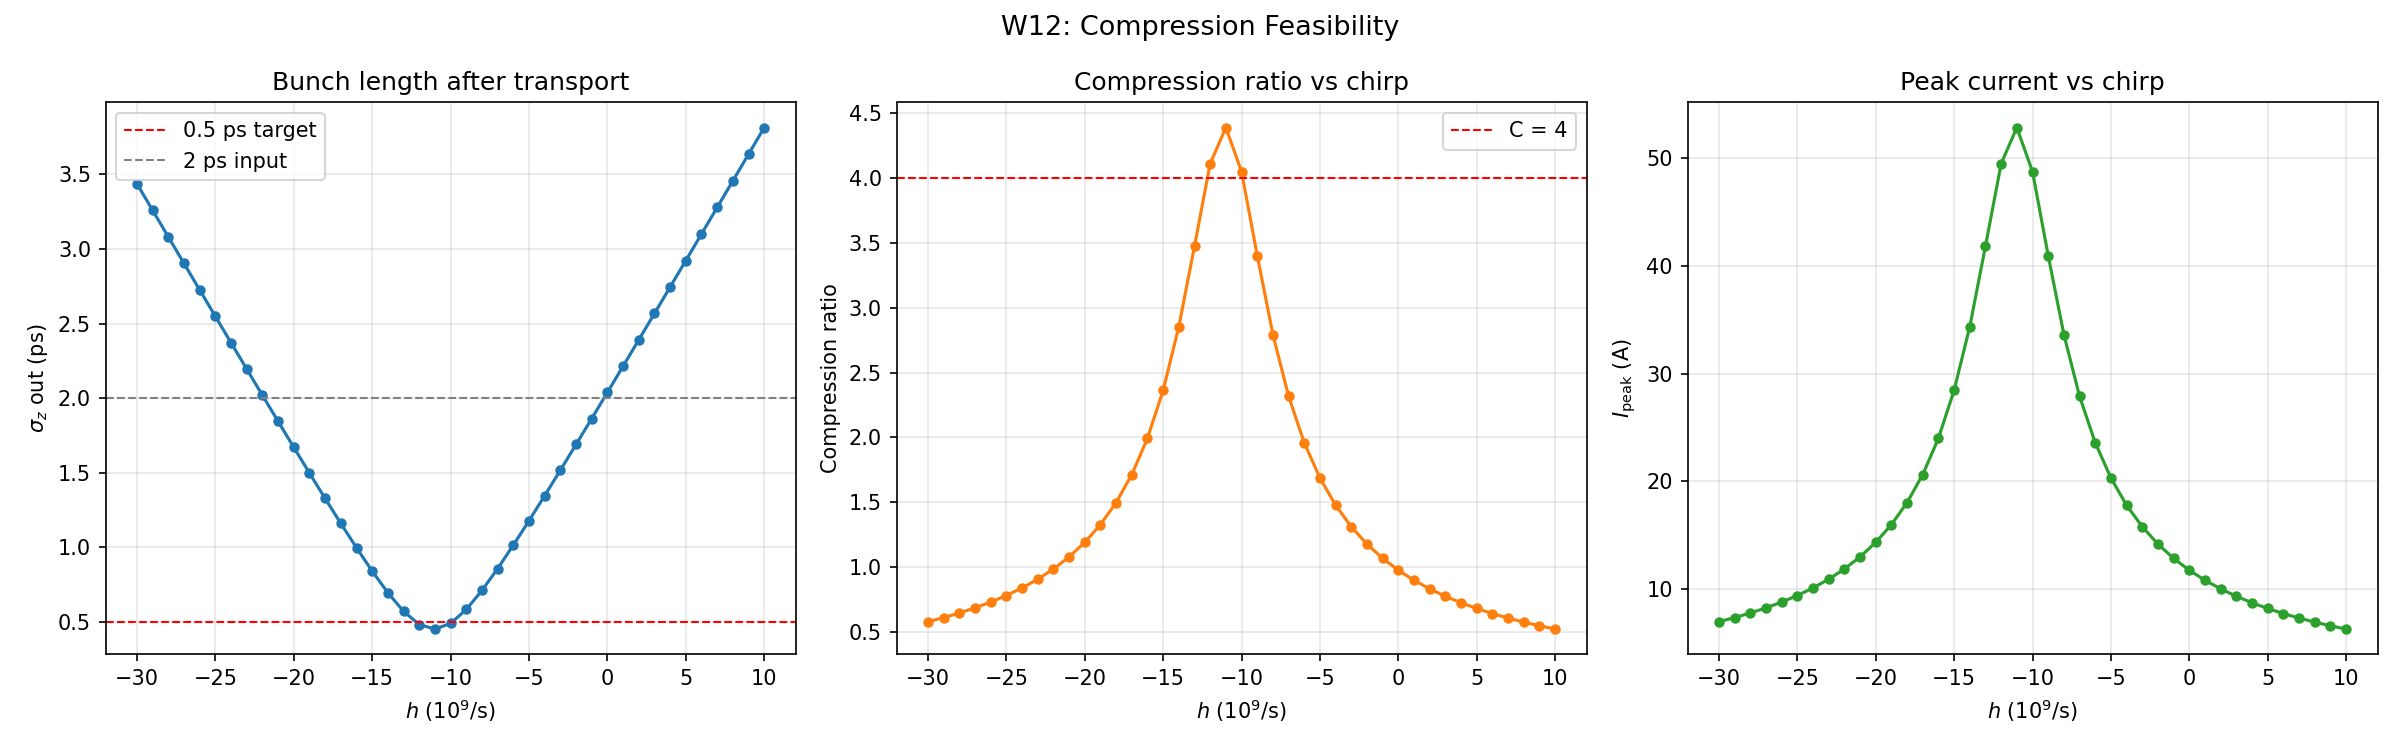
\includegraphics[width=\textwidth]{results/R2/R2_compression_curve}
  \caption{Bunch compression factor vs chirp rate (W12 Part~A).
    Analytical and COSY map propagation agree closely.  The compression
    floor ($\approx$\SI{0.45}{ps}) prevents reaching \SI{0.5}{ps}
    at practical chirp values.}
  \label{fig:compression}
\end{figure}

\begin{figure}[p]
  \centering
  
\includegraphics[width=0.85\textwidth]{results/params_05ps/W7/mse_comparison}
  \caption{Stage~11 MSE comparison across optimisers and emittance
    points (W6/W7 data).  COSY FIT (gradient-based DA) achieves the
    lowest MSE at $\varepsilon_n = 8$ and 14; NM is competitive.
    Both glyfada configurations fail by orders of magnitude.}
  \label{fig:opt_mse}
\end{figure}


\begin{thebibliography}{9}
\bibitem{weinberg2025}
  M.~Weinberg, A.~Fisher, and R.~Li,
  ``Design of the UH Mark V Free Electron Laser,''
  arXiv:2510.14061v1, Table~I.
\end{thebibliography}

\end{document}
